% !TEX TS-program = pdflatex
% !TEX encoding = UTF-8 Unicode

% This is a simple template for a LaTeX document using the "article" class.
% See "book", "report", "letter" for other types of document.

\documentclass[11pt]{report} % use larger type; default would be 10pt

\usepackage[utf8]{inputenc} % set input encoding (not needed with XeLaTeX)

%%% Examples of Article customizations
% These packages are optional, depending whether you want the features they provide.
% See the LaTeX Companion or other references for full information.

%%% PAGE DIMENSIONS
\usepackage{geometry} % to change the page dimensions
\geometry{a4paper} % or letterpaper (US) or a5paper or....
% \geometry{margin=2in} % for example, change the margins to 2 inches all round
% \geometry{landscape} % set up the page for landscape
%   read geometry.pdf for detailed page layout information

\usepackage{graphicx} % support the \includegraphics command and options
\usepackage{subfiles}
% \usepackage[parfill]{parskip} % Activate to begin paragraphs with an empty line rather than an indent

%%% PACKAGES

\usepackage{pdfpages}

\usepackage{booktabs} % for much better looking tables
\usepackage{array} % for better arrays (eg matrices) in maths
\usepackage{paralist} % very flexible & customisable lists (eg. enumerate/itemize, etc.)
\usepackage{verbatim} % adds environment for commenting out blocks of text & for better verbatim
\usepackage{subfig} % make it possible to include more than one captioned figure/table in a single float
% These packages are all incorporated in the memoir class to one degree or another...

%%% HEADERS & FOOTERS
\usepackage{fancyhdr} % This should be set AFTER setting up the page geometry
\pagestyle{fancy} % options: empty , plain , fancy
%\renewcommand{\headrulewidth}{0pt} % customise the layout...
\renewcommand{\sectionmark}[1]{\markright{#1} }
\lhead{Martin Simon Haugaard}
\rhead{\rightmark}
%\cfoot{center of the footer!}
%\lfoot{}\cfoot{\thepage}\rfoot{}
%\renewcommand{\headrulewidth}{0.4pt}
\renewcommand{\footrulewidth}{0.4pt}

%\fancyhf{}
%\fancyhead[C]{Some centered header}
\fancyfoot[C]{\thepage}

%%% SECTION TITLE APPEARANCE
\usepackage{sectsty}
\allsectionsfont{\sffamily\mdseries\upshape} % (See the fntguide.pdf for font help)
% (This matches ConTeXt defaults)

%%% ToC (table of contents) APPEARANCE
\usepackage[nottoc,notlof,notlot]{tocbibind} % Put the bibliography in the ToC
\usepackage[titles,subfigure]{tocloft} % Alter the style of the Table of Contents
\renewcommand{\cftsecfont}{\rmfamily\mdseries\upshape}
\renewcommand{\cftsecpagefont}{\rmfamily\mdseries\upshape} % No bold!

%%% END Article customizations

%%% The "real" document content comes below...

\title{Brief Article}
\author{The Author}
%\date{} % Activate to display a given date or no date (if empty),
         % otherwise the current date is printed 

\begin{document}
\tableofcontents
\newpage

\addcontentsline{toc}{section}{First Project}
\addcontentsline{toc}{subsection}{Report}
\rhead{First Project - Report}
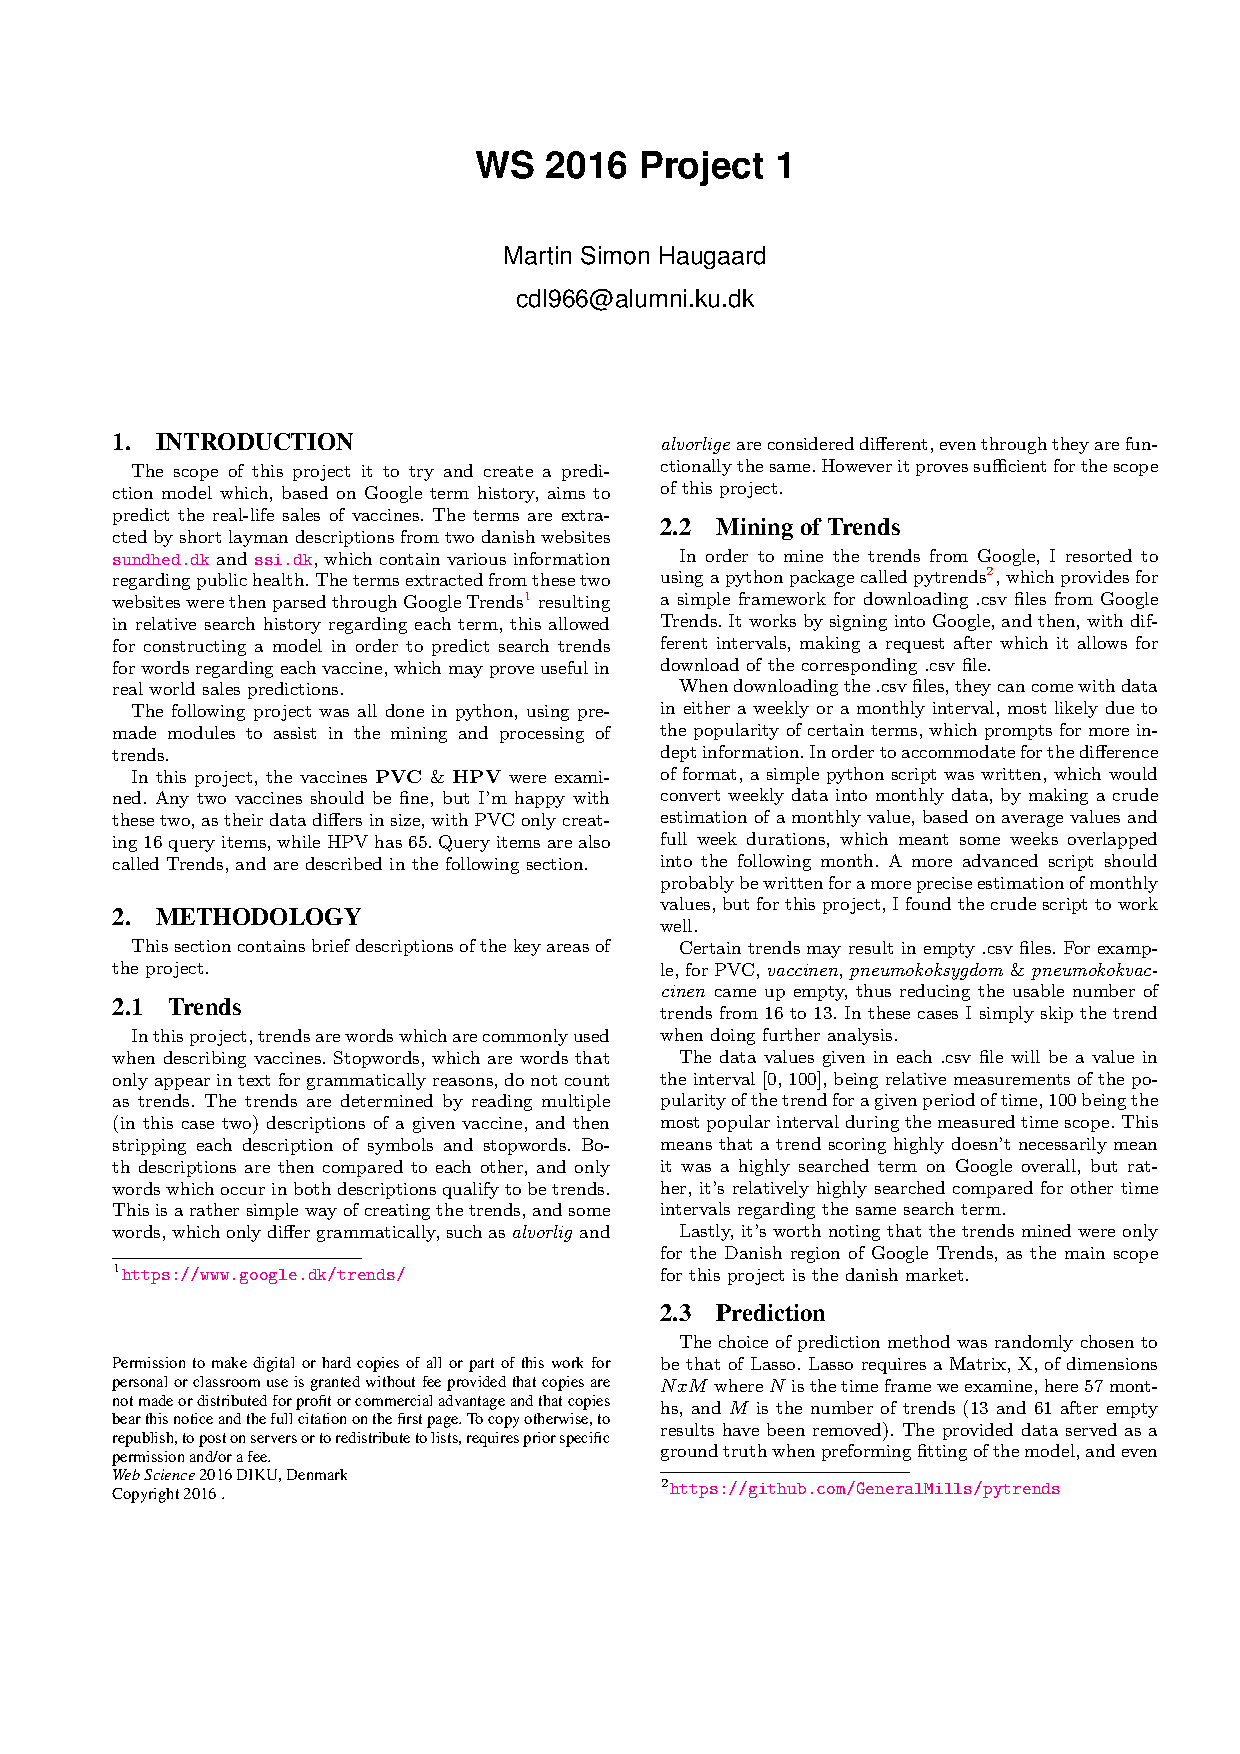
\includepdf[scale=0.9,pages=-,pagecommand={\pagestyle{fancy}}]{Handin_1/template-WS-project1}

\rhead{First Project - Received Peer-Review}
\addcontentsline{toc}{subsection}{Received Peer-Review}
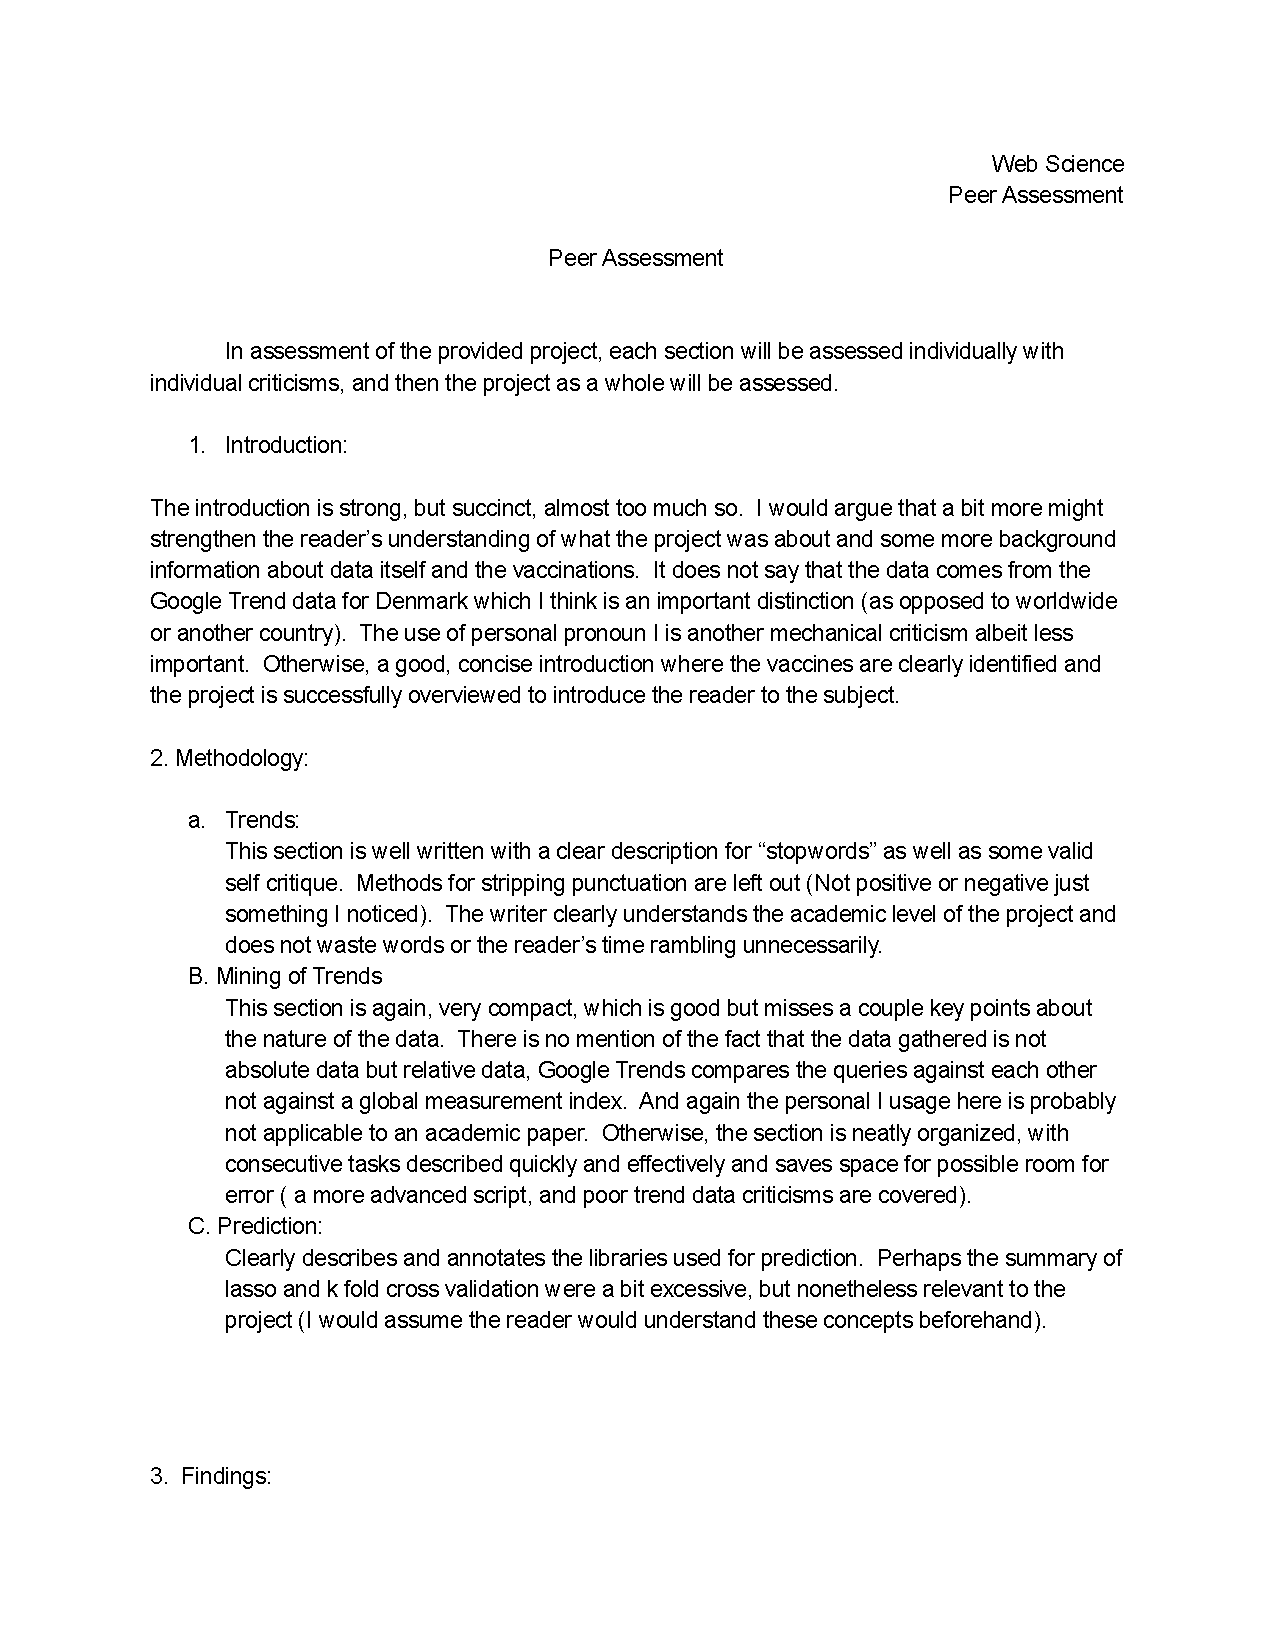
\includepdf[scale=0.9,pages=-,pagecommand={\pagestyle{fancy}}]{WebSciencePeerAssessment1.pdf}

\rhead{First Project - Amendment List}
\addcontentsline{toc}{subsection}{Amendment List}
\section*{Amendment List}
\begin{description}
\item[Extend introduction to strengthen reader's understanding]\hfill\\{The Introduction was extended to mention the websites used, and is not a short recap of the entire project in a single section.}
\item[Explain Google Trends data for Denmark]\hfill\\{While intuative to know, I've added a brief sentence covering this, in section \textbf{2.2 Mining of Trends}.}
\item[Personal pronoun \textit{'I'} not applicable academic paper]\hfill\\{I can see the logic behind this claim, but I've chosen to keep using 'I', as it's a one person project, and using other pronouns such as "we" or "our" may confuse the reader into thinking it was a group effort, and avoiding any such pronoun altogether would result in hard to read language. Also, I've stayed true to using 'I' throughout the project, which is my main concern, keeping it continuous.}
\item[Trends - Missing methods for stripping punctuation]\hfill\\{I find this trivial, and hence not included in a paper. I've made clear that I'm only interested in words as trends, hence it should be obvious that special characters are stripped.}
\item[Mining of Trends - Nature of Data Explanation, Not absolute but relative]\hfill\\{Also worth noting, and as such a paragraph has been introduced in the section in question.}
\item[Summary of lasso and k-fold cross validation bit excessive.]\hfill\\{I don't think it's too excessive to explain these points, as it's the main feature of the project. I would argue that the reader has an academic background, but k-fold and lasso (which I've only mentioned by name) was new to me at the beginning of this course, thus worth including.}
\item[Findings - Writing too compact, more explanation might be helpful]\hfill\\{
%\begin{description}\item[Frequency data was left out of the findings]{}
%\item[Might be difficult to read for people who have not taken course in a while]{}\end{description}
In order to accommodate this, I've expanded slightly on RMSE, as I find it to be the least intuitive part of what I've written.}
\item[Little expansion upon the connection between the predictive dataset and observed dataset]\hfill\\{I find the connection given in Section \textbf{4. Conclusions} to be sufficient.}
\item[Elaborate on the connection between the frequency output from Google and the predictive model]\hfill\\{I've expanded slightly in the conclusions to explain that not every term may weigh equally in the real world, but they all have the same weight in the model.}
\item[Critical thinking section might be helpful]\hfill\\{Changes made in conclusion section now serves as critical thinking as well.}
%                           What do the predictions mean? How do outliers affect the predictive model? What other factors might be involved?
\item[More expansions upon the findings could strengthen the project enormously]\hfill\\{As before, the findings / conclusions section has been expanded as pr request from other amendments, so I find this fulfilled.}
\end{description}
\newpage

\rhead{First Project - Written Peer-Review}
\addcontentsline{toc}{subsection}{Written Peer-Review}
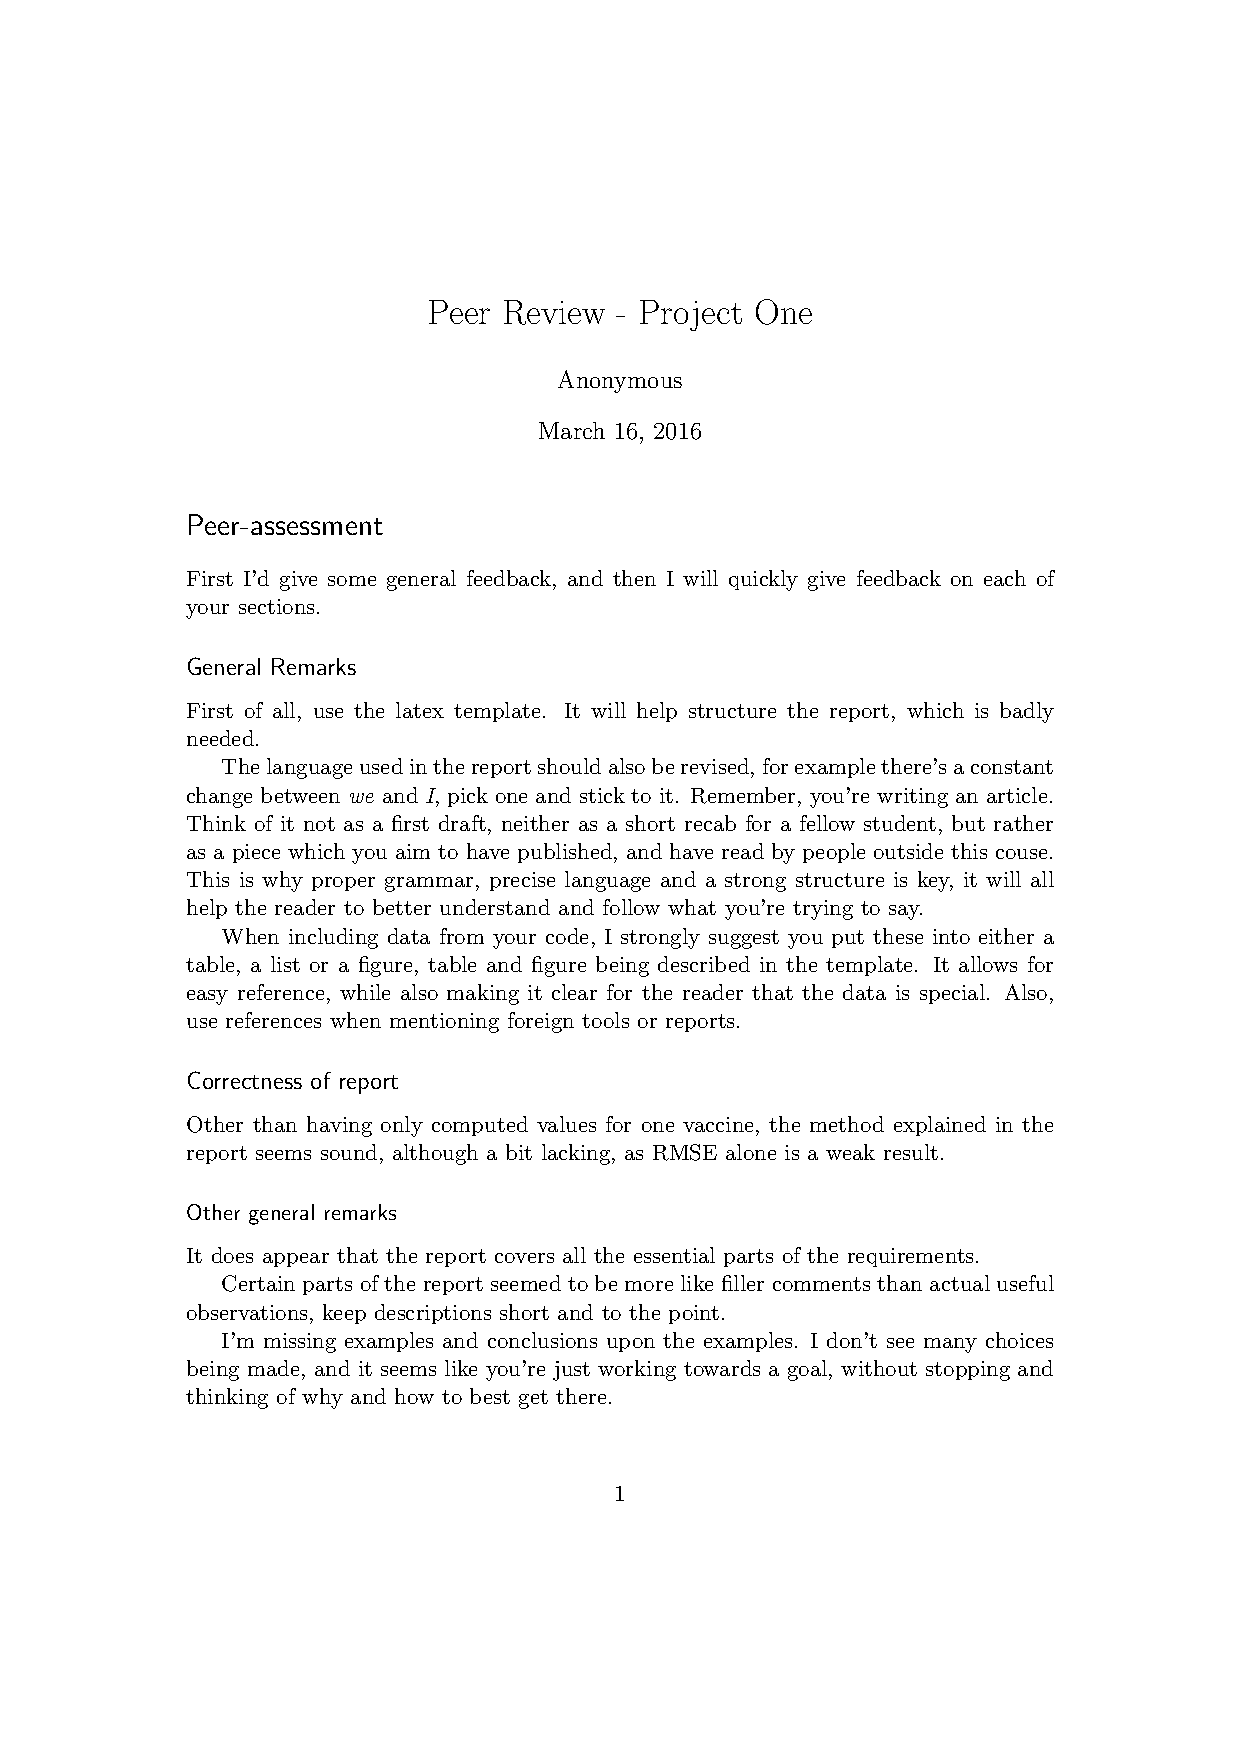
\includepdf[scale=0.9,pages=-,pagecommand={\pagestyle{fancy}}]{Peer_Review_1/review}

\rhead{Second Project - Report}
\addcontentsline{toc}{section}{Second Project}
\addcontentsline{toc}{subsection}{Report}
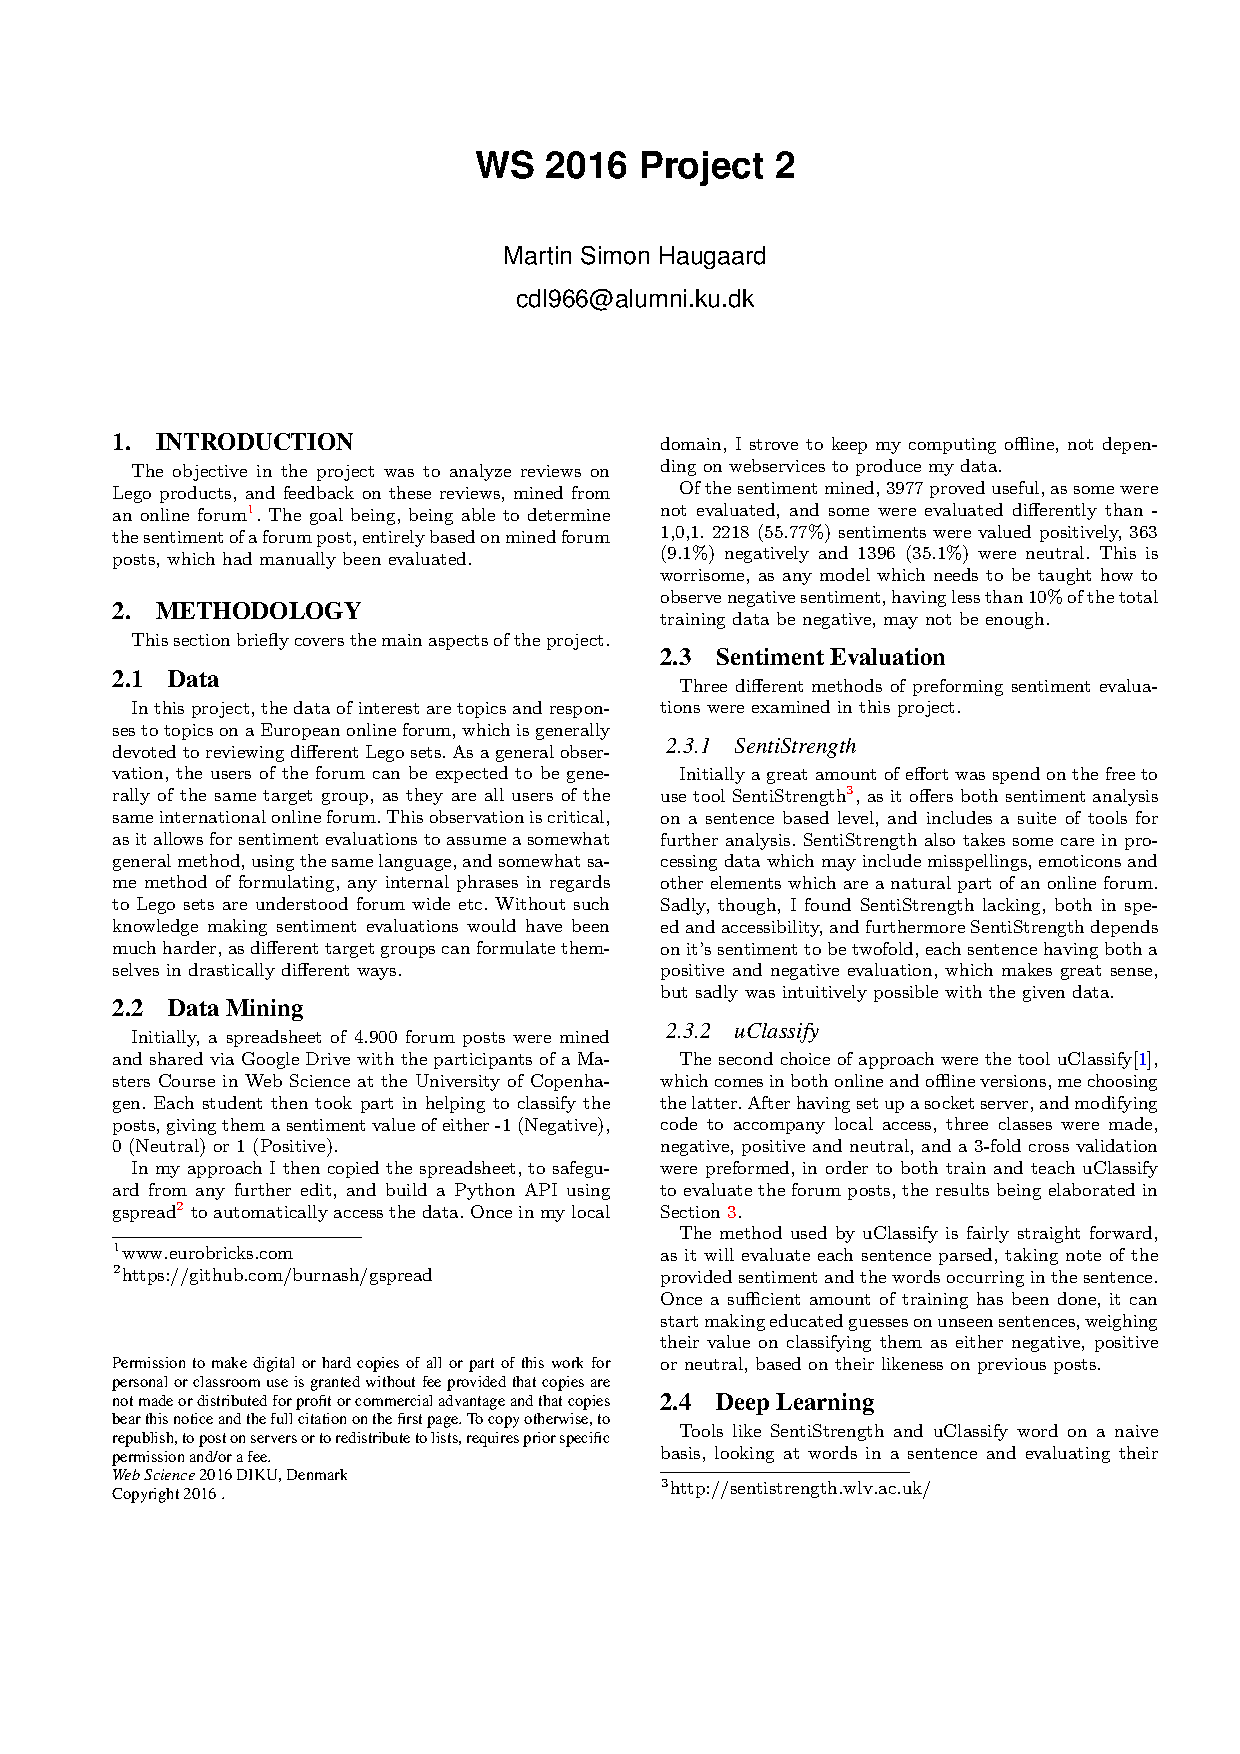
\includepdf[scale=0.9,pages=-,pagecommand={\pagestyle{fancy}}]{Handin_2/template-WS-project1}

\rhead{Second Project - Received Peer-Review}
\addcontentsline{toc}{subsection}{Received Peer-Review}
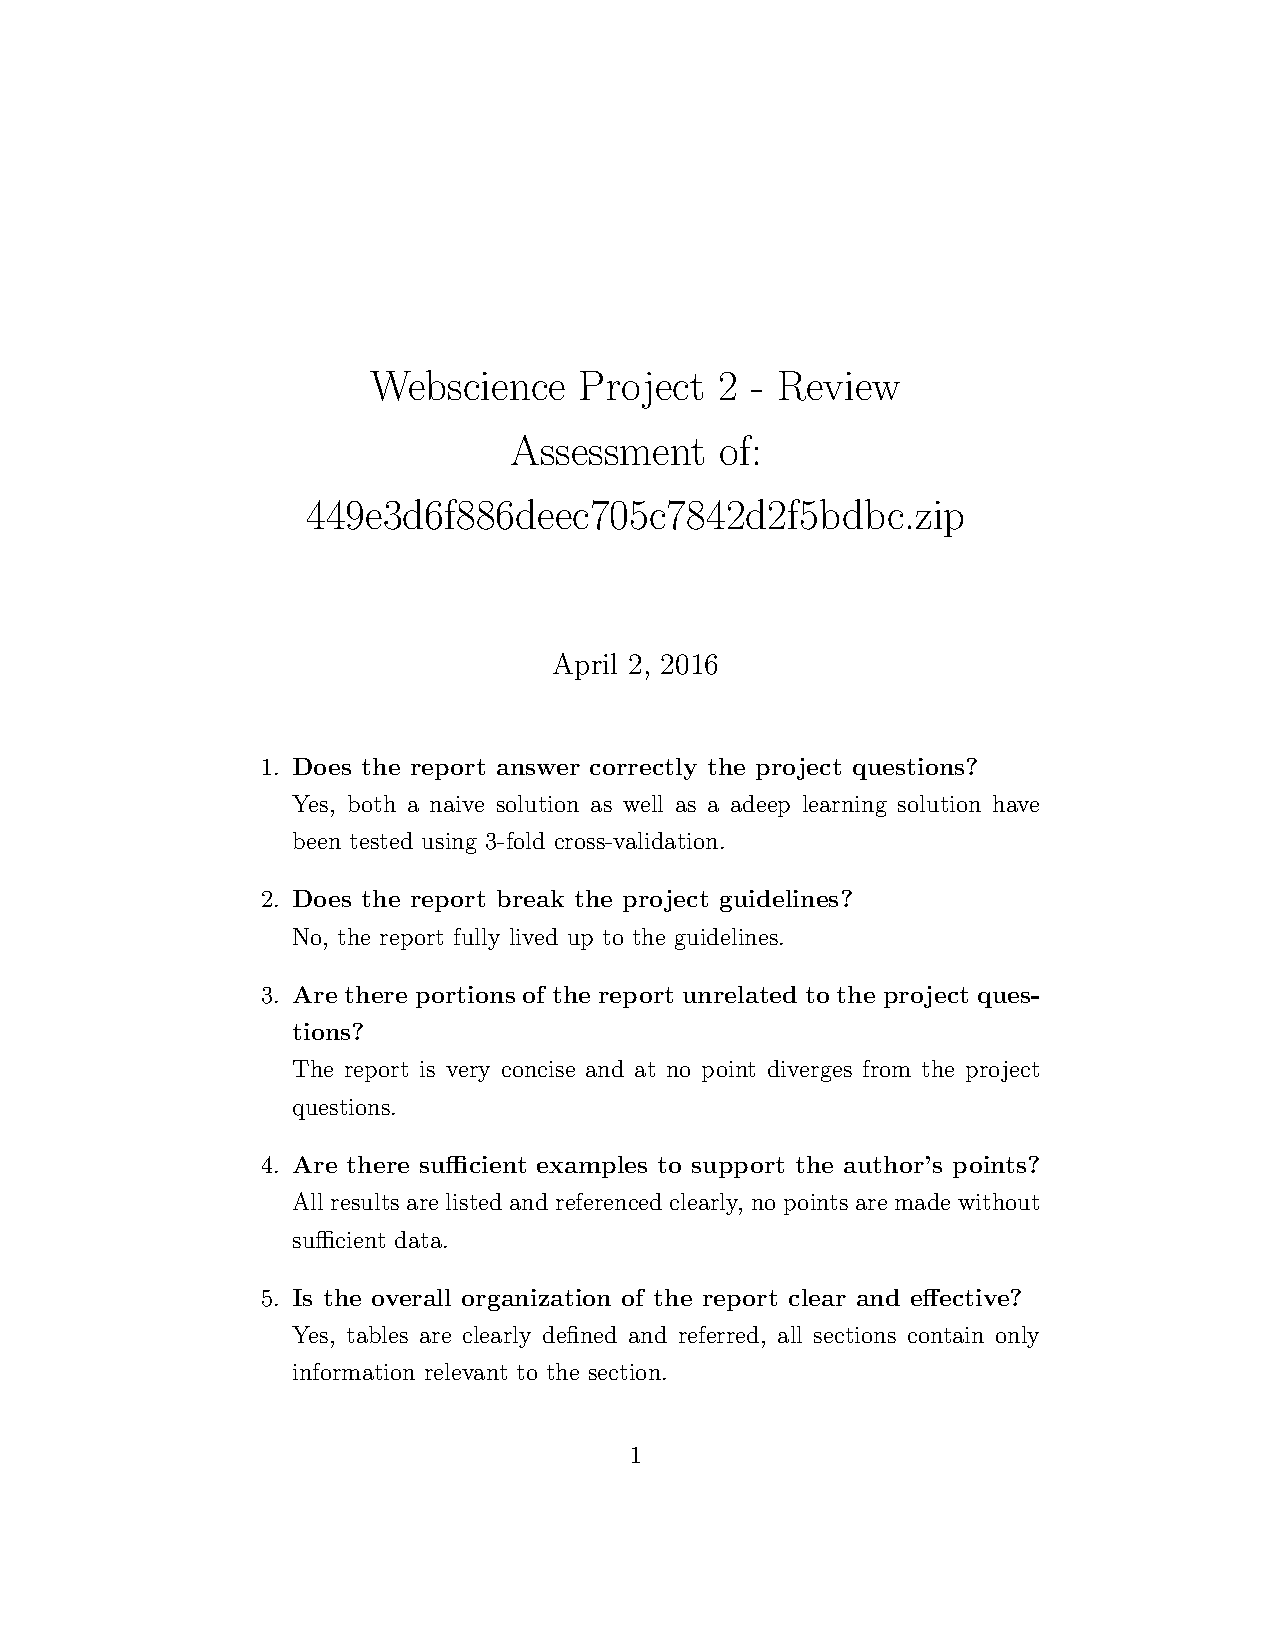
\includepdf[scale=0.9,pages=-,pagecommand={\pagestyle{fancy}}]{review.pdf}

\rhead{Second Project - Amendment List}
\addcontentsline{toc}{subsection}{Amendment List}
\section*{Amendment List}
\begin{description}
\item[How many percent is positive labels in our data]\hfill\\{This is now covered in section \textbf{2.2 Data Mining}}
\item[55\% positive diminishes the result of 60\% and 67\%.]\hfill\\{I would argue not, as I'm concerned about success-rates. Only correct predictions count, meaning any incorrect prediction should lower my result, still having 67\% is quite good.}
\item[Description of the data in the beginning would be nice]\hfill\\{A new section \textbf{2.1 Data} were introduced.}
\item[Sections should never be empty]\hfill\\{Section \textbf{2 Methodology} how has brief introduction.}
\item[Short intro for \textbf{2.2 Sentiment Evaluation}]\hfill\\{Short intro added.}
\item[Remove "TEMPLATE"/"Keep anonymous" from title"]\hfill\\{Removed, and now holds name of author.}
\item[Appendix A is missing (Just Appendix)]\hfill\\{Fixed, now refers to appendix, no A.}
\end{description}

\rhead{Second Project - Written Peer-Review}
\addcontentsline{toc}{subsection}{Written Peer-Review}

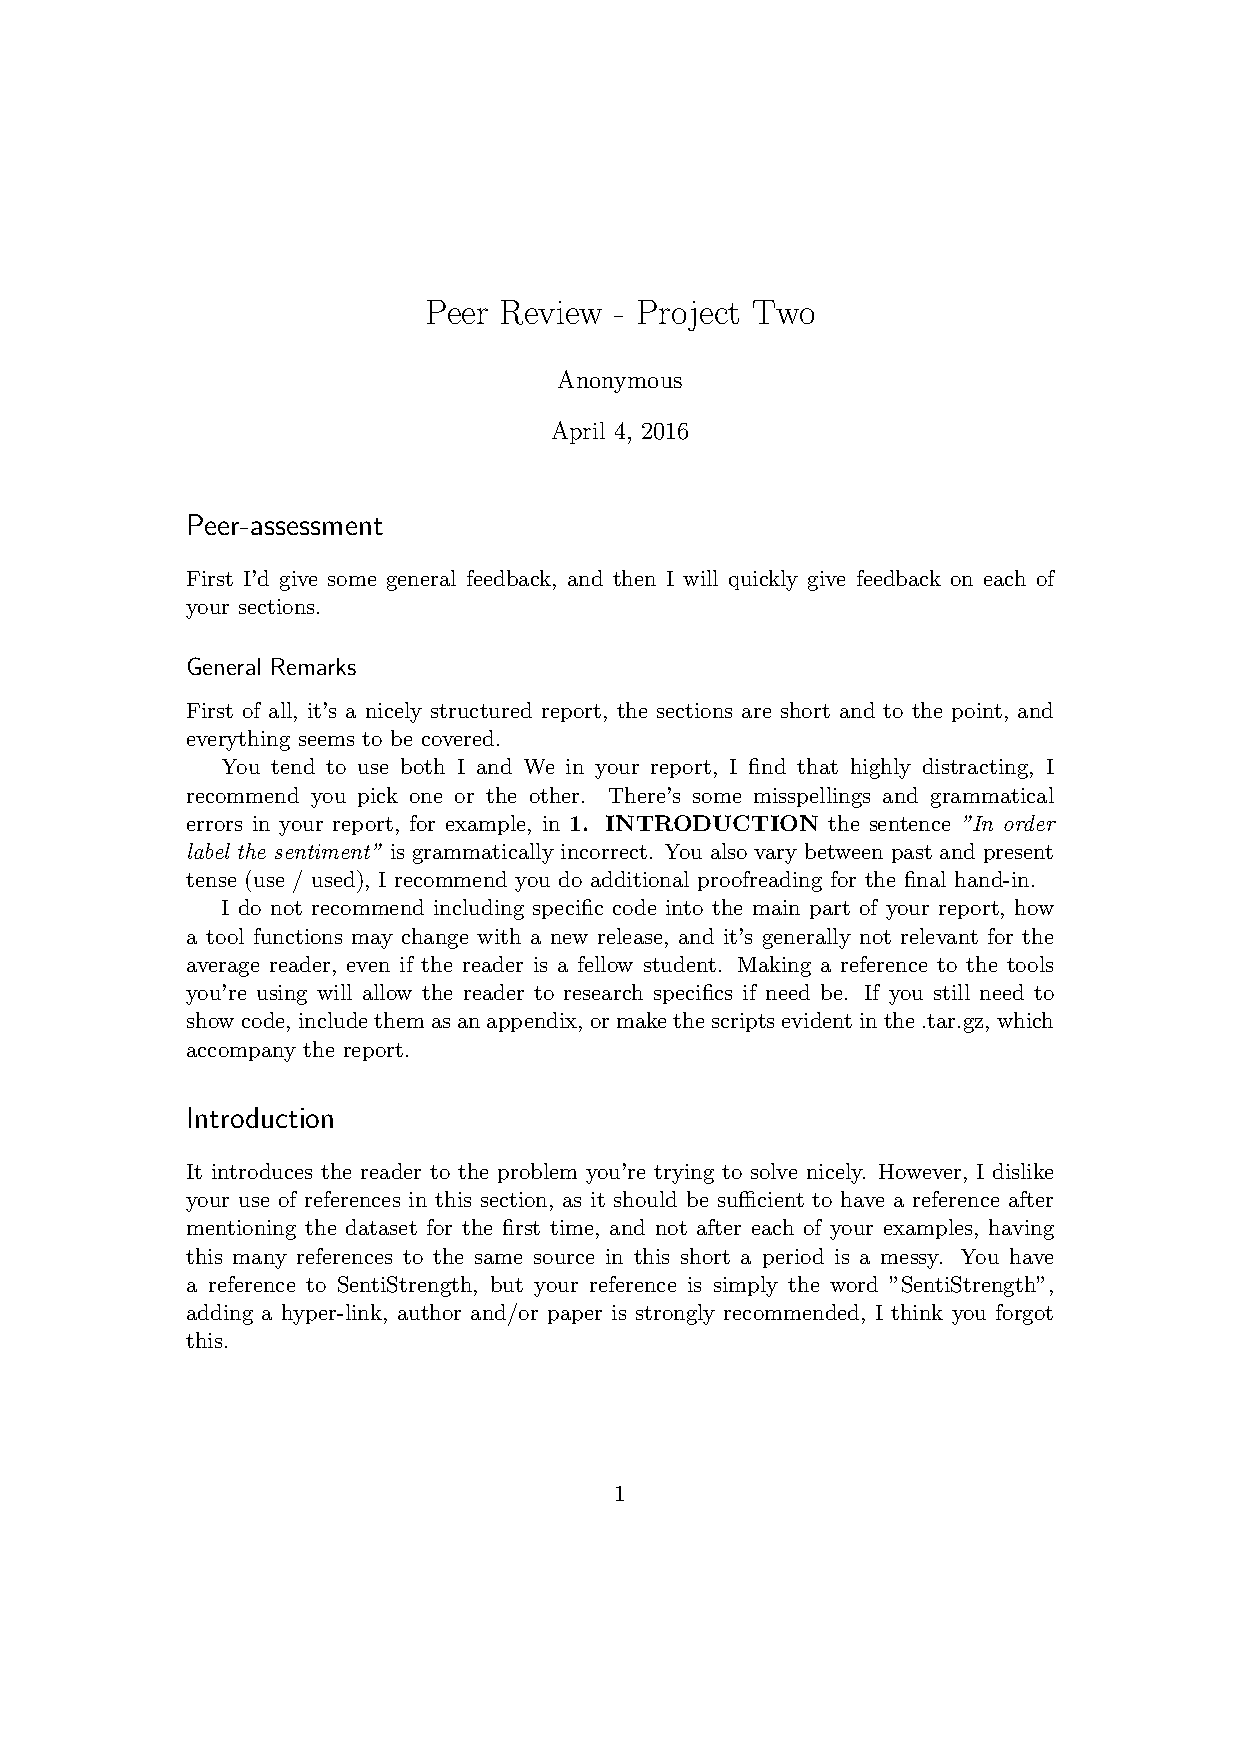
\includepdf[scale=0.9,pages=-,pagecommand={\pagestyle{fancy}}]{Peer_Review_2/review}

\end{document}
